% !TeX spellcheck = nl_NL
\chapter{Data verwerving}

% inleiding van dit hoofdstuk, wat ga ik allemaal bespreken
In dit hoofdstuk wordt de verwerving van de data toegelicht. Er wordt eerst enkele belangrijke specificaties van de gebruikte toestellen besproken. Vervolgens worden de gehanteerde programma's doorgenomen op vlak van gebruikte data en type \gls{nn}. Het hoofdprogramma wordt in de Python-programmeertaal geschreven. Deze taal werd gekozen door de veelvuldige toepassingsmogelijkheden binnen \gls{ml}. Tot slot wordt de dataverwerving van de benchmark zelf ge\"illustreerd en besproken hoe de data opgeslagen wordt.

% Verkennen te gebruiken software
\section{Verkennen van software}
% in welke mate vertel ik hier al over pyrenn????
% uitleggen wat tensorflow is en hoe ik het gebruik. = tensorflowlite

% Verkennen devices
\section{Verkennen edge-devices}
	% welke benodigdheden zijn er om programma's te runnen; coral dev: tflite
	% aanvullende data zoals cpu% kost,...
	
% subsectie: structuur runV4
\section{Structuur programma}
In deze sectie wordt de structuur van het hoofdprogramma besproken. De belangrijkste onderdelen van de programma's worden toegelicht. Zo wordt er weergegeven hoe de verschillende \gls{nn}-modellen opgebouwd zijn en op welke data ze worden toegepast voor zowel het trainen als het uitvoeren. De benchmark bevat in totaal 10 verschillende subprogramma's. Elk van deze is een neuraal netwerk met een zekere complexiteit bedoeld voor weide variatie aan applicaties. Van de 10 subprogramma's kunnen er zes van gecategoriseerd worden als regressie en vier als classificatie. Voor elk subprogramma wordt er uitgelegd hoe het model wordt opgesteld, hoe het getraind wordt en hoe het uiteindelijk uitgevoerd wordt. Voor de benchmark is vooral het uitvoeren van de modellen van belang. Het opstellen en trainen van een \gls{nn} is een eenmalige taak en hoeft bijgevolg niet op edge-devices gebeuren.


	\subsection{Regressie subprogramma's}
	Voor de regressie subprogramma's werd er gekozen om gebruik te maken van pyrenn\footnote{Meer info over pyrenn is te vinden op https://pyrenn.readthedocs.io/en/latest/index.html}. Dit is een toolbox voor zowel Python als Matlab. Deze laat op een heel eenvoudige manier \gls{nn} trainen en uitvoeren. De pyrenn-toolbox heeft 2 dependencies of afhankelijkheden in Python. Deze zijn de gekende pandas en numpy packages.  De volgende subprogramma's worden opgesteld met behulp van de pyrenn-voorbeelden. 
		% Verwerving data pyrenn
		% Opstellen programma's
		\subsubsection{Programma 1: compair}
		Het eerste subprogramma is een \textit{compressed air storage system} of een samengedrukte lucht opslagsysteem. Het systeem met drie verschillende inputs en 2 gewenste outputs. De praktische werking wordt verduidelijkt in figuur \ref{fig:compairPraktijk} maar wordt in deze thesis verder niet op in gegaan.
			
		\begin{figure}
			\centering
			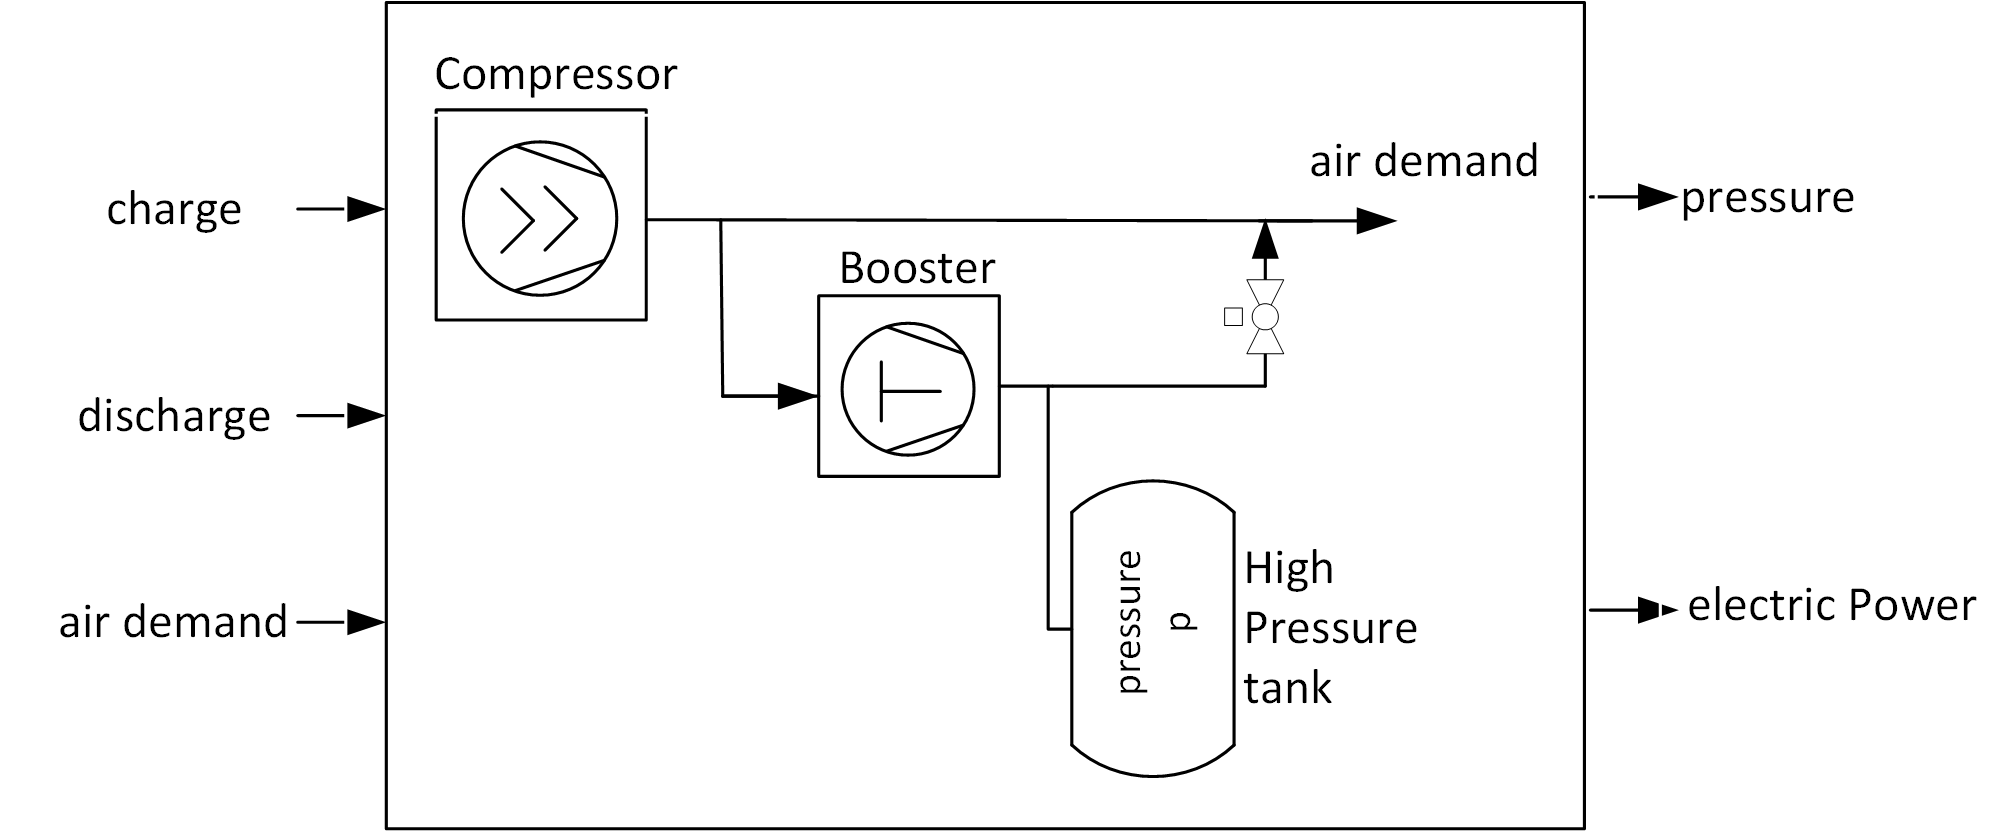
\includegraphics[width=120mm]{afbeeldingen/compairPraktijk.PNG}
			\caption{Praktische betekenis van het compair-subprogramma. \\Afbeelding te vinden op https://pyrenn.readthedocs.io/en/latest/examples.html\\ Website werd geraadpleegd op 10/04/2020.}
			\label{fig:compairPraktijk}
			%bron: https://medium.com/machine-learning-bites/machine-learning-decision-tree-classifier-9eb67cad263e
		\end{figure}
	
			\paragraph{Aanmaken en trainen model}
			Voor dit subprogramma werd er gewerkt met een dataset voorzien door Pyrenn zelf. Deze dataset levert in totaal 960 data inzendingen voor de inputs en outputs. Hiervan zijn er 480 inzendingen voorzien voor trainen en 480 voor testen van het model. In tabel \ref{Tab:dataVoorbeelden} kan u een voorbeeld vinden van \'e\'en datalijn.
			%\numblock{\fbox{Testing, 1,2,3 testing a box}}
			
			\begin{table}[]
				
				\centering
				\begin{tabular}{@{}lllllll@{}}
					\toprule
					subprogramma                   & index & P1       & P2 & P3  & Y1       & Y2  \\ \midrule
					\multicolumn{1}{l|}{compair}   & 464   & 0        & 1  & 0.8 & 7        & 8.4 \\
					\multicolumn{1}{l|}{friction}  & 14    & -3       &    &     & -0,29148 &     \\
					\multicolumn{1}{l|}{narendra4} & 80    & -0,54404 &    &     & -0,45803 &     \\
					\multicolumn{1}{l|}{pt2}       & 208   & -7,96923 &    &     & -0,44761 &     \\ \bottomrule
				\end{tabular}
				\label{Tab:dataVoorbeelden}
				\caption{Voorbeelden van de gebruikte data voor regressiemodellen.}
			\end{table}

		\subsubsection{Programma 2: friction}
		\subsubsection{Programma 3: narendra4}
		\subsubsection{Programma 4: pt2}
		\subsubsection{Programma 5: P0Y0-narendra4}
		\subsubsection{Programma 6: gradient}
		
		
	\subsection{Classificatie subprogramma's}
		% verwerving data verscheidene programmas'
		% uitleg elk programma
		% uitleg tensorflow en keras
		\subsubsection{Programma 7: FashionMNIST}
		\subsubsection{Programma 8: NumberMNIST}
		\subsubsection{Programma 9: catsVSdogs}
		\subsubsection{Programma 10: Image Recognition}
	\subsection{Conversie naar TFLite}
% uitleggen ophalen data zoals cpu% en tijddata
\section{Uitvoeren metingen}


% Hoe opslaan data
\section{Opslaan van data}
	% gebruik maken van unieke filenaam